\part{Appendici}
\chapter{Appendici manoscritte}
\section{Legame fra la mancanza dell'autovalore $m_z=0$ di spin fotonico e la
proprietà di trasversalità dell'onda elettromagnetica}
\label{sec:autovalore0fotone}
La ``gauge'' di Coulomb del potenziale elettromagnetico
$\vec{\nabla}\cdot \vec{A} = 0$ vincola l'onda elettromagnetica ad avere una
polarizzazione trasversale. COnsideriamo ad esempio un'onda piana che si propaga
lungo l'asse $z$ e sia del tipo
\begin{equation}
  \vec{A} = \Re\left\{A_0\vec{e}\exp\left[ i\left( kz-\omega t \right)
  \right]\right\}
\end{equation}
dove $\vec{e}$ è il vettore unitario di componenti reali $(e_x,e_y,e_z)$ di
polarizzazione. Si avrà allora:
\[
  \vec{\nabla}\cdot\vec{A} = \frac{\partial A}{\partial z}= 0 \Rightarrow e_z =
  0\Rightarrow \vec{e}\cdot\vec{k} = 0
\]
dove $\vec{e}\cdot\vec{k}=0$ esprime proprio la condizione di trasversalità
dell'onda.

Per una direzione di propagazione lungo $z$, la soluzione più generale di onda
piana sarà del tipo
\begin{equation}
  \Re\left\{ \hat{x}A_{0_x}\exp\left[ i\left( kz-\omega t \right) \right] +
  \hat{y}A_{0_y}\exp\left[ i\left( kz - \omega t + \delta \right) \right] \right\}
\end{equation}
dove $\hat{x}$ e $\hat{y}$ sono i versori degli assi $x$ e $y$ e dove $\delta$
indica lo sfasamento relativo delle due componenti $A_x$ e $A_y$ di $\vec{A}$.
Nel caso in cui $\delta=0$ si torna ad una polarizzazione lineare, mentre nel
caso in cui $\delta=\pm\pi/2$ e $A_{0_x}=A_{0_y}=A_0$ si ottiene una
polarizzazione circolare (levogira o destrogira). In quest'ultimo caso si avrà
corrispondentemente:
\begin{equation}
  \vec{A} = \hat{x}A_0\cos\left( kz-\omega t \right) \pm \hat{y}A_0\sin\left(
  kz-\omega t \right)
\end{equation}
e $\vec{A}$ potrà anche scriversi nella forma
\[
  \Re\left\{ \hat{x}A_{0}\exp\left[ i\left( kz-\omega t \right) \right] \pm
  \hat{y}A_{0}\exp\left[ i\left( kz - \omega t \right) \right] \right\}
\]

Potremo in particolare avere
\[
  \vec{A} = \Re\left\{ \sqrt{2}A_0 \vec{e}_L \exp\left[ i\left( kz-\omega t \right) \right] \right\}
\]
se la polarizzazione è levogira, oppure
\[
  \vec{A} = \Re\left\{ \sqrt{2}A_0 \vec{e}_L \exp\left[ i\left( kz-\omega t \right) \right] \right\}
\]
se la polarizzazione è destrogira, dove
\[
  \vec{e}_L \equiv \frac{\hat{x} + i\hat{y}}{\sqrt{2}}\qquad\vec{e}_R \equiv \frac{\hat{x} - i\hat{y}}{\sqrt{2}}
\]

I due versori di polarizzazione circolare $\hat{e}_L$ e $\hat{e}_R$ sono tali
che una rotazione attorno all'asse $z$
\[
  \hat{x}'=\hat{x}\cos(\varphi) + \hat{y}\sin\left( \varphi \right),\qquad
  \hat{y}'=-\hat{x}\sin\left( \varphi \right) + \hat{y}\cos\left( \varphi
  \right)
\]
provocherà le rispettive trasformazioni
\begin{equation}
  \begin{dcases}
	\vec{e'}_L&=\vec{e}_L\exp\left( -i\varphi \right)\\
	\vec{e'}_R&=\vec{e}_R\exp\left( +i\varphi \right)\\
    \vec{e'}_z&=\vec{e}_z = 0
  \end{dcases}
\end{equation}

Ciò va confrontato col fatto che \textit{$\vec{A}$ rappresenta anche la funzione
d'onda quantistica del fotone} e che una rotazione attorno all'asse $z$ sarà
corrispondentemente rappresentata dall'operatore $\exp\left( iJ_z\varphi/\hslash
\right)$ dove $J_z$ è la componente $z$ del momento angolare totale del fotone.
In teoria i possibili autovalori di $J_z$ sono $-1,0,+1$ dove $\pm1$ sono
semplicemente autovalori di spin del fotone (in quanto il momento angolare
orbitale del fotone non può avere una componente longitudinale alla sua quantità
di moto). È immediato allora vedere che le due polarizzazioni $\vec{e}_L$ e
$\vec{e}_R$ corrispondono ai due stati di spin del fotone con autovalori $\pm1$
lungo $z$, mentre la \textit{mancanza} di una polarizzazione longitudinale
dell'onda corrisponde alla \textit{mancanza} di uno stato di spin fotonico con
autovalore $0$ lungo $z$ (infatti possiamo scrivere $\vec{e'}_z =
\vec{e}_z\exp\left( i0 \right)$.
\section[Decadimento del caone +]{Decadimento del mesone $K^+$}
\label{ch:mesonek}
Il mesone $K^+$, detto caone +, ha tempo di vita media
$\tau_k\simeq1,23\times10^{-8}$ sec e può decadere debolmente in 2 o 3 pioni.
\begin{align}
  K^+ &\rightarrow \pi^+ + \pi^0         & (R \simeq 21\%)\label{eq:a1}\\
  K^+ &\rightarrow \pi^+ + \pi^+ + \pi^0 & (R \simeq 5,6\%)\\
  K^+ &\rightarrow \pi^+ + \pi^0 + \pi^0 & (R \simeq 1,7\%)
\end{align}

Un discorso simmetrico varrebbe per il caone $K^-$, solo che avendo stranezza $s
= -1$ non fa in tempo a decadere perch viene assorbito da un nucleo secondo la
reazione:
\begin{align*}
  K^- + N &\rightarrow \pi + \Lambda^0\\
  K^- + N &\rightarrow \pi + \Sigma
\end{align*}
cioè trasforma un nucleone in un iperione. $K^+$ invece avendo $s=+1$ subisce
uno scattering elastico con i nuclei circostanti.

La presenza di canali con 2 e 3 pioni finali implica che non viene conservata la
parità. Questo non fu compreso subito, si pensava vi fossero due tipi di $K^+$,
denominati $\theta^+$ e $\tau^+$, con parità intrinseche opposte: $\theta^+$
doveva decadere in due pioni, $\tau^+$ in tre pioni.

Ci si accorse però che i dati non erano compatibili con l'assegnazione di due
diversi valori di parità intrinseca. Ciò diede lo spunto nel 1965 ai fisici
cinesi Lie e Yang di suggerirenuna verifica diretta della simmetria per
inversione spazione nei processi devoli. Tale verifica venne effettuata l'anno
dopo per i processi$\beta$ con il decadimento del Co$^{60}$.

Consideriamo il decadimento \eqref{eq:a1}. Supponendo $K^+$ a riposo e sapendo
che tutti gli elementi hanno spin nullo, si ha che $l =0$. Se applichiamo
l'operatore parità otterremo:
\begin{equation}
  P\Ket{\pi^+,\pi^0} = \eta_\pi^2(-1)^2\Ket{\pi^+,\pi^0}=(+1)\Ket{\pi^+,\pi^0}
\end{equation}
quindi lo stato finale ha parità $+1$.

Se invece consideriamo i decadimenti di $K^+$ in 3 pioni, con $K^+$ a riposo, il
momento angolare totale dei tre pioni si può scrivere come
\[
  \vec{J} = \vec{L}_{12} + \vec{L}_3
\]
dove $\vec{L}_{12}$ è il momento angolare dei primi due pioni rispetto al centro
di massa ed $\vec{L}_3$ è il momento angolare del terzo pione rispetto ai primi
due.

Dato che il momento angolare iniziale è zero, lo stato finale sarà autostato di
$\vec{J}$ con autovalore $j =0$. Allora dovrà risultare $j = j_{\text{min}} =
\abs{l_{12}-l_3} =0\Rightarrow l_{12} = l_3$.

Ricordando che la parità intrinseca del pione è $-1$ avremo:
\[
  P\Ket{3\pi} = \eta^3_\pi(-1)^{l_{12}}(-1)^{l_3}\Ket{3\pi} =
  \eta^3_\pi(-1)^{2l_3}\Ket{3\pi} = \eta^3_\pi\Ket{3\pi} = (-1)\Ket{3\pi}
\]

Visto che lo stesso $K^+$ può decadere in due stati con parità opposte
\textit{il decadimento non conserva la parità}.

Il caone $K^+$ decade anche in canali leptonici e semileptonici, per esempio
\begin{equation}
  \left.
  \begin{split}
	K^+ &\rightarrow e^+ + \nu\\
	K^+ &\rightarrow \pi^0 + e^+ + \nu
  \end{split}
  \right\rbrace\,\text{gli stati finali non hanno parità definita}
\end{equation}
e analogamente
\begin{equation}
  \left.
  \begin{split}
	K^+ &\rightarrow e^+ + \bar{\nu}\\
  K^+ &\rightarrow \pi + e^+ + \bar{\nu}
  \end{split}
  \right\rbrace
\end{equation}
\[
  \Ket{e^-,\bar{\nu}} = CP\Ket{e^+,\nu}
\]
Per il canale leptonico $\Ket{\pi^0,e^-,\bar{\nu}}=CP\Ket{\pi^0,e^+,\nu}$.

\section[Decadimento del caone zero]{Decadimento del mesone $K^0$}
Il caone $K^0$ ha stranezza $s = +1$, mentre $\bar{K}^0$ ha $s =-1$, quindi
$K^0$, pur essendo elettricamente neutro, è diverso da $\bar{K}^0$.

Se applichiamo l'operatore coniugazione di carica $C$, a meno di una costante di
fase arbitraria, otterremo:
\begin{equation}
  C\Ket{K^0} = \Ket{\bar{K}^0} \neq \Ket{K^0}
\end{equation}
ovvero $CP\Ket{K^0} \neq \Ket{K^0}$.

Storicamente questo risultato incontrò una seria difficoltà di principio. $K^0$
e $\bar{K}^0$ perdendo stranezza possono decadere in uno stesso stato non
leptonico che risolta autostato dell'operatore $CP$, come avviene in 
\begin{align*}
  K^0       &\rightarrow \pi^+ + \pi^-\\
  \bar{K}^0 &\rightarrow \pi^+ + \pi^-
\end{align*}

Ma se ciò è vero, come è possibile parlare di simmetria rispetto a $CP$ e di
conservazione del numero quantico associato a $CP$, dato che n\'e $K^0$ n\'e
$\bar{K}^0$ vengono prodotti come autostati di $CP$?

Nel 1955 Gell-Mann e Pais suggerirono un modo di risolvere tale difficoltà:
$K^0$ e $\bar{K}^0$ non erano le vere particelle che subivano decadimento.

Consideriamo $K^0$ e $\bar{K}^0$ a riposo e indichiamo con $\Ket{K^0}$ e
$\Ket{\bar{K}^0}$ i loro stati iniziali. Poich\'e hanno parità intrinseca $(-1)$
potremo scrivere
\[
  P\Ket{K^0} = (-1)\Ket{K^0}\qquad P\Ket{\bar{K}^0} = (-1)\Ket{\bar{K}^0}
\]

Definiamo $C$ in modo tale che $C\Ket{K^0} = - \Ket{\bar{K}^0}$, così che
$CP\Ket{K^0} = \Ket{\bar{K}^0}$. Dato che i due stati iniziali differiscono per
l'operatore di stranezza, definiamo uno spazio interno di Hilbert a due
dimensioni, in cui i due stati $\Ket{K^0}$ e $\Ket{\bar{K}^0}$ costituiscono una
base ortonormale. In questo spazio si può introdurre un'altra base costituita
dai vettori
\begin{align}
  \Ket{K_1^0} &= \frac{1}{\sqrt{2}}(\Ket{K^0} + \Ket{\bar{K}^0}\\
  \Ket{K_2^0} &= \frac{1}{\sqrt{2}}(\Ket{K^0} - \Ket{\bar{K}^0}
\end{align}

I nuovi vettori di base hanno la proprietà di essere autostati di $C$:
\begin{align*}
  C\Ket{K_1^0} &= -\Ket{K_1^0}\\
  C\Ket{K_2^0} &= +\Ket{K_2^0}
\end{align*}
Inoltre avendo entrambi parità $p=-1$ saranno entrambi autostati di $CP$
\begin{align*}
  CP\Ket{K_1^0} &= \Ket{K_1^0}\\
  CP\Ket{K_2^0} &= -\Ket{K_2^0}
\end{align*}
D'altra parte nessuno dei due è autostato della stranezza, quindi questi due
vettori non coincidono con gli stati iniziali di produzione di $K^0$ e
$\bar{K}^0$. $K_1^0$ e $K_2^0$ hanno un ruolo fondamentale nell'interazione
responsabile del decadimento devole.

\breaknote

Consideriamo l'hamiltoniana $\mathcal{H}$ nello spazio definito dai due stati
$\Ket{K^0}$ e $\Ket{\bar{K}^0}$ e scriviamola nella sua forma completa
\[
  \mathcal{H} = \mathcal{H}_0 + \mathcal{H}_d
\]
dove l'hamiltoniana debole $\mathcal{H}_d$ è un termine non hermitiano
responsabile del decadimento.

Poich\'e $\mathcal{H}_d$ non conserva la stranezza $[S,\mathcal{H}] =
[S,\mathcal{H}_d] \neq 0$ e quindi gli autostati di $\mathcal{H}$ non potranno
più essere autostati della stranezza.
Quindi $\Ket{K^0}$ e $\Ket{\bar{K}^0}$ non potranno più risultare autostati di
$\mathcal{H}$ (anche se sono inizialmente autostati di $\mathcal{H}_0$).

Assumendo che $\mathcal{H}_d$ sia invariante rispetto a $CP$ potremo costruire
autostati simultanei di $\mathcal{H}$ e $CP$ che sono $\Ket{K_1^0}$ e
$\Ket{K_2^0}$, infatti non ci sono altri autostati di $CP$ nello spazio
considerato.

È chiaro che questo autostati non saranno degeneri, cioè non avranno lo stesso
autovalore di energia, perch\'e altrimenti risulterebbe che anche $\Ket{K^0}$
e $\Ket{\bar{K}^0}$ sono autostati di $\mathcal{H}$. Da ciò traiamo che $\Ket{K_1^0}$ e
$\Ket{K_2^0}$ sono gli unici autostati di $\mathcal{H}$.

Sremmo arrivati allo stesso risultato se, come Gell-Mann e Pais, avessimo
supposto $\mathcal{H}_d$ invariante rispetto a $C$ piuttosto che, come abbiamo
invece fatto noi, rispetto a $CP$.

Riepilogando potremmo dunque porre:
\begin{align}
  H\Ket{K_1^0} &= \left( m_1c^2 - i\frac{\Gamma_1}{2} \right)\Ket{K_1^0}\\
  H\Ket{K_2^0} &= \left( m_2c^2 - i\frac{\Gamma_2}{2} \right)\Ket{K_2^0}
\end{align}
dove $\Gamma_1$ e $\Gamma_2$ sono le larghezze del livello energetico
rispettivamente di $K_1^0$ e $K_2^0$ e dove, poich\'e gli autovalori
dell'energia devono essere diversi deve risultare
\[
  m_1c^2 - i\frac{\Gamma_1}{2}\neq m_2c^2 - i\frac{\Gamma_2}{2}
\]

Le particelle rappresentate da $\Ket{K_1^0}$ e $\Ket{K_2^0}$ sono quindi le vere
particelle a massa complessa definita e vita media definita che subiscono il
decadimento (dove per massa complessa si intende l'autovalore complesso di
energia diviso $c^2$.

Gli stati finali in cui queste particelle decadono saranno effettivamente
distinguibile perch\'e dovranno risutlare autostati di $CP$ con autovalori
differenti (perch\'e $CP$ si conserva).

Per esempio, se $\Ket{f_1}$ e $\Ket{f_2}$ sono due stati finali associati a
$K_1^0$ e $K_2^0$ si avrà:
\begin{equation*}
  \left.
  \begin{split}
    CP\Ket{f_1} &= f_1\\
	CP\Ket{f_2} &= -f_2
  \end{split}\right\rbrace
  \Rightarrow f_1\neq f_2
\end{equation*}

Considerando in particolare i canali di decadimento non leptonici si vede che
$\Ket{f_1}$ può contenere due soli pioni, mentre $\Ket{f_2}$ deve contenere come
minimo tre pioni, in altri termini
\begin{equation*}
  \begin{split}
	K_1^0 &\rightarrow \pi^+ + \pi^- \qquad K_2^0 \nrightarrow \pi^+ + \pi^-\\
	K_1^0 &\rightarrow \pi^0 + \pi^0 \qquad K_2^0 \nrightarrow \pi^0 + \pi^0
  \end{split}
\end{equation*}
infatti, per la casistica di Bose-Einstein, $CP\Ket{\pi^+,\pi^-}
=\Ket{\pi^+,\pi^-}$ è autostato dei $CP$ con autovalore $+1$ in quanto $\pi^+$ e
$\pi^-$ possono considerarsi due bosoni identici in un diverso stato di carica e
applicare loro $CP$ significa scambiare tutte le coordinate dei due bosoni,
compresa la coordinata di carica elettrica. Rilsuterà invece
\[
  \begin{split}
	K_1^0 &\nrightarrow \pi^0 + \pi^0 + \pi^0\\
	K_2^0 &\rightarrow \pi^0 + \pi^0 + \pi^0\\
	K_2^0 &\rightarrow \pi^+ + \pi^- + \pi^0
  \end{split}
\]
infatti ricordando che tre pioni con momento angolare nulla hanno parità $-1$ e
considerando che $C\Ket{\pi^0} = (+1)\Ket{\pi^0}$ otteniamo che
\[
  CP\Ket{3\pi} = -C\Ket{3\pi} = -\Ket{3\pi}
\]

Un analogo risultato si può ottenere anche per lo stato finale $\pi^+ + \pi^- +
\pi^0$ nella sua configurazione più probabile, che è quella con\footnote{Qui gli
  appunti sono poco leggibili e non si è sicuri dell'uguaglianza fra i due
autovalori. Pagina 101 dell'appendice con calligrafia differente. [NdT]} $l_{12}
= l_3 = 0$. Questa configurazione comporta che si abbia
\begin{equation*}
  \begin{split}
	P\Ket{\pi^+,\pi^-} &= \Ket{\pi^+, \pi^-}\\
	C\Ket{\pi^+,\pi^-} &= CP\Ket{\pi^+, \pi^-} = \Ket{\pi^+, \pi^-}
  \end{split}
\end{equation*}
e da ciò segue che
\begin{equation}
  CP\Ket{\pi^+, \pi^-, \pi^0} = P\Ket{\pi^+, \pi^-,\pi^0}= -\Ket{\pi^+,
  \pi^-,\pi^0}
\end{equation}

Questo modo diverso di decadere di $K_1^0$ e $K_2^0$ ha anche una ripercussione
sulle loro costanti di disintegrazione $\lambda_1$ e $\lambda_2$. Se si applica
la regola d'oro di Fermi e si calcola la densità di stati finali, questa sarà
maggiore per lo stato finale costituito da due pioni rispetto a quello
costituito da tre pioni, infatti partendo da una stessa energia iniziale,
l'impulso dei pioni nello stato costituito da due pioni è ovviamente maggiore di
quello nello stato cotituito da tre pioni e\footnote{Anche qui gli appunti si
  leggono male, ma suppongo che il simbolo corretto sia proprio $\rho$ o al
limite una sua variante spesso usata $\varrho$.}
\[
  \frac{\text{d}N}{\text{d}\rho} = \text{densità di stati finali} = \rho^2
\]
di conseguenza $\lambda_1 \gg\lambda_2$ e quindi $\tau_1\ll\tau_2$.

Supponiamo che all'istante $t=0$ venga prodotto un fascio di mesoni $K^0$ con
una  data velocità. Nel sistema di riferimento solidale col fascio potremmo
scrivere lo stato iniziale di ogni $K^0$ come
\[
  \Ket{K^0} = \frac{1}{\sqrt{2}}\left( \Ket{K_1^0} + \Ket{K_2^0} \right)
\]

Al generico istante $t$ questo $K^0$ si sarà evoluto nello stato
\[
  \Ket{K^0(t)} = \frac{1}{\sqrt{2}}\left(
  \Ket{K_1^0}e^{-im_1c^2t/\hslash}e^{-t/2\tau_1}+\Ket{K_2^0}e^{-im_2c^2t/\hslash}e^{-t/2\tau_2} \right)
\]

Di conseguenza, se $t$ soddisfa la condizione che $\tau_1\ll t\ll\tau_2$ allora
la componente $K_1^0$ avrà avuto il tempo di decadere e l'intensità del fascio
si sarà dimezzata riducendosi a quella di un puro fascio di particelle $K_2^0$.
Avremo allora
\[
  \Ket{K^0(t)}\simeq \frac{1}{\sqrt{2}}\Ket{K_2^0}e^{-im_2c^2t/\hslash} =
  \frac{1}{\sqrt{2}}\left( \frac{1}{\sqrt{2}}\Ket{K^0} -
  \frac{1}{\sqrt{2}}\Ket{\bar{K}^0} \right)e^{-im_2c^2t/\hslash}
\]
quindi dopo un tempo pari a $t$ circa un quarto dei caoni iniziali si saranno
trasformati in anticaoni con stranezza  $-1$, di conseguenza partendo da un
fascio non in grado di produrre iperoni otterremo dopo un certo tempo un fascio
in grado di produrre iperoni.

Questo effetto di conversione di $K^0$ in $\bar{K}^0$ è stato confermato
dell'esperienza. Si è potuto constatare che solo metà dei caoni iniziali
presentava una vita media molto breve $\tau_1\simeq 0,9\cdot 10^{-10}$ sec
decadendo prevalentemente in due pioni vicino al punto di produzione mentre
l'altra metà del fascio viveva per $\tau_2\simeq 5,2\cdot 10^{-8}$ sec,
decadendo in altri modi, tra cui quello in tre pioni, a notevole distanza dalla
sorgente.

Facendo passare il fascio residuo a vita lunga attraverso un gas si è misurata
la frequenza di produzione degli iperoni e da questa si è risaliti all'intensità
di $\bar{K}^0$ nel fascio residuo.

Inoltre studiando l'andamento generale dell'intensità dei $\bar{K}^0$ in
funzione del tempo si è determinato $\abs{\delta} = \abs{m_2-m_1}$.

Per capire come sia possibile ricavare $\abs{\delta}$ indichaimo con $I_0$
l'intensità iniziale del fascio di caoni e con $I(t)$ e $\bar{I}(t)$ le
intensità rispettivamente dei $K^0$ e dei $\bar{K}^0$ all'istante $t$, misurate
nel sistema di riferimento solidale col fascio. Avremo
\[
  \bar{I}(t) = I_0\abs{\braket{\bar{K}^0|K^0(t)}}^2
\]
dove $\abs{\braket{\bar{K}^0|K^0(t)}}^2$ e $\abs{\braket{K^0|K^0(t)}}^2
$ sono le probabilità che una singola particella del fascio si manifesti
all'istante $t$ rispettivamente come $\bar{K}^0$ o $K^0$ e si ha
\[
  \begin{split}
	\abs{\braket{K^0|K^0(t)}}^2 &= \abs{\frac{1}{\sqrt{2}}\braket{K_1^0|K^0(t)}
	+ \frac{1}{\sqrt{2}}\braket{K_2^0|K^0(t)}}^2=\\
	&= \abs{\frac{1}{2}e^{im_1c^2t/\hslash}e^{-\lambda_1t/2} +
	\frac{1}{2}e^{im_2c^2t/\hslash}e^{-\lambda_2t/2}}^2=\\
    &=\frac{1}{4}\left[ e^{\lambda_1t} + e^{\lambda_2t} + 2\exp\left(
	  \frac{-\lambda_1t - \lambda_2t}{2}
	\right)\cos\left( \frac{c^2\abs{\delta m}t}{\hslash} \right)\right]
  \end{split}
\]
analogamente
\[
  \abs{\braket{\bar{K}^0|K^0(t)}}^2=\frac{1}{4}\left[ e^{\lambda_1t} + e^{\lambda_2t} + 2\exp\left(
  \frac{-\lambda_1t - \lambda_2t}{2}
  \right)\cos\left( \frac{c^2\abs{\delta m}t}{\hslash} \right)\right]
\]

In queste formule $\abs{\delta m}$ gioca un ruolo essenziale, infatti se
risultasse $c^2\abs{\delta m}/\hslash > \lambda_1$ si avrebbe una rapida
oscillazione tra $K^0$ e $\bar{K}^0$ di frequenza $\omega = c^2\abs{\delta
m}/\hslash$ e la presenza dei $\bar{K}^0$ dovrebbe essere osservata già prima
del decadimento del fascio a vita breve. Ciò non ha invece alcun riscontro
sperimentale e i dati suggersicono invece $\abs{\delta m} c^2
\simeq3,5\cdot10^{-6}$eV che è dello stesso ordine di grandezza di $\Gamma_1$.

Si noti quanto questa differenza di massa è piccola rispetto alla massa dei
caoni, infatti\footnote{Questi dati sono presi direttamente dagli appunti,
  tuttavia non hanno molto senso rispetto a quento detto qualche rigo sopra.
[NdT]}
\[
  \frac{\abs{\delta m}}{m} =
  \frac{3,5\cdot10^{-12}\text{MeV}}{5\cdot10^2\text{MeV}}\simeq
  7\cdot10^{-15}
\]

\breaknote

Ci sono due tipi di caoni, uno a vita breve $K_1^0$ e uno a lunga vita $K_2^0$,
che può decadere in canali semileptonici
\[
  \begin{split}
	K_2^0 &\rightarrow \pi^- + \bar{e} + \nu\qquad (\bar{e}=e^+,\mu^+)\\
    K_2^0 &\rightarrow \pi^+ + e + \bar{\nu} \qquad (e = e^-,\mu^-)
  \end{split}
\]
con $\Delta q= \Delta s$.

Il primo decadimento è attribuibile solo a $K^0$ mentre il secondo solo a
$\bar{K}^0$.

Indichiamo con $\Gamma(\pi^-, \bar{e}, \nu)$ e con $\Gamma(\pi^+, e, \bar{\nu})$
le larghezze parziali relative a questi decadimenti semipleptonici
\[
  \Ket{K_2^0} = \frac{1}{\sqrt{2}}\left( \Ket{K^0} - \Ket{\bar{K}^0}\right)
\]

La simmetria rispetto a $CP$ richiede che si abbia
\begin{equation}
  \frac{\Gamma(\pi^-,\bar{e},\nu)}{\Gamma(\pi^+,e,\bar{\nu})}=1
  \label{eq:g}
\end{equation}

Fino ad ora abbiamo supposto che tale simmetria sia rispettata nei decadimenti
dei caoni neutri, tuttvia nel 1964 si è scoperto che tale simmetria viene
violata anche se in misura piccolissima.

Per tenere conto di questa variazione indichiamo con $K_L^0$ il caone a lunga
vita e con $K_S^0$ il caone a vita breve.

Anche $K_L^0$ può decadere in due pioni, sebbene con un rapporto di diramazione
\[
  R(K_L^0\rightarrow 2\pi)\simeq 0,3\%
\]
con una larghezza parziale tale che
\[
  \frac{\Gamma(K_L^0\rightarrow 2\pi)}{\Gamma(K_S^0\rightarrow 2\pi)}\simeq
  2,3\cdot10^{-3}
\]

Analagomante si trovò che i due modi di decadimento del tipo
\[
  \begin{split}
	K^0_L &\rightarrow \pi^- + \bar{e} + \nu\\
	K^0_L &\rightarrow \pi^+ + e + \bar{\nu}
  \end{split}
\]
non presentavano larghezze parziali identiche come si sarebbe dovuto avere dalla
\eqref{eq:g}.

\chapter{Allegati presenti negli originali}
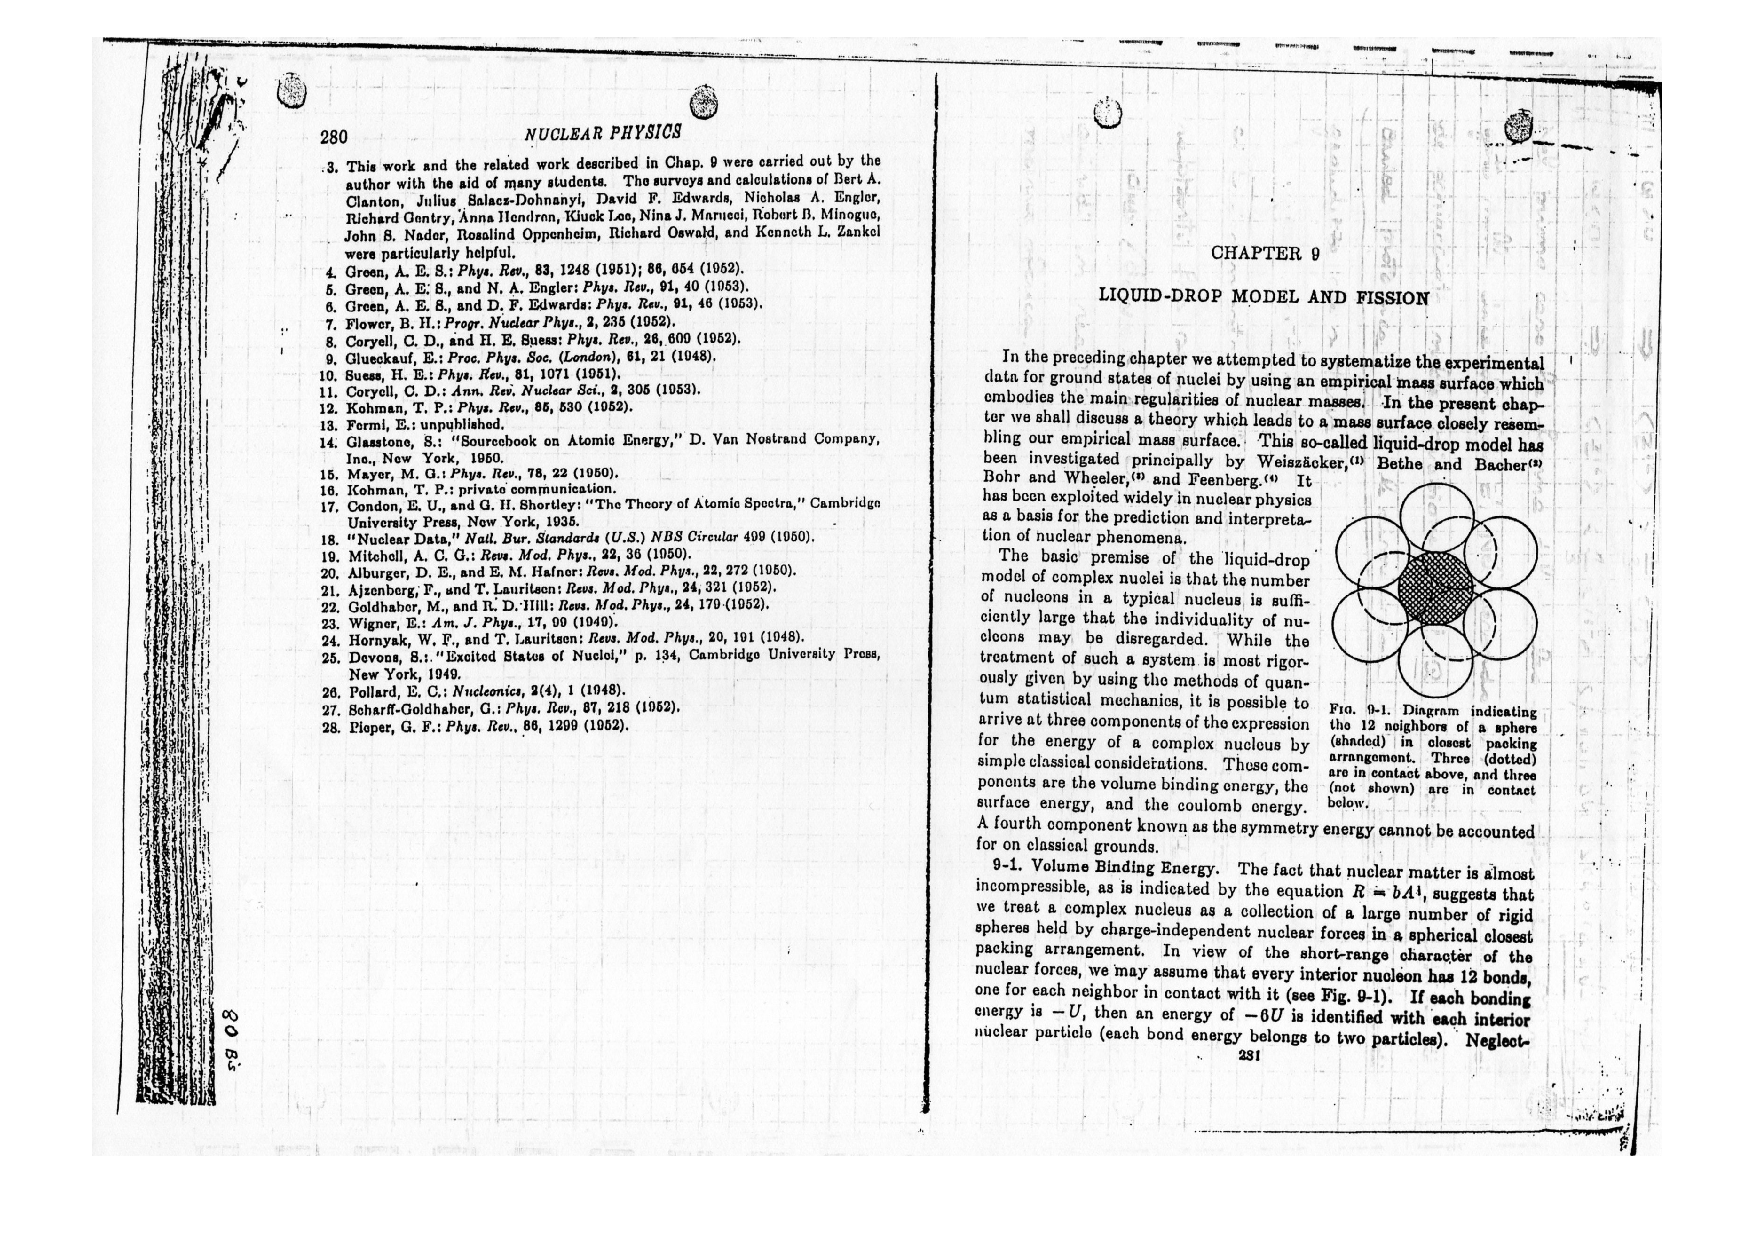
\includepdf[landscape,fitpaper=true,addtotoc={1,section,1,Allegato\
1,allegato_1}]{allegati/1.pdf}
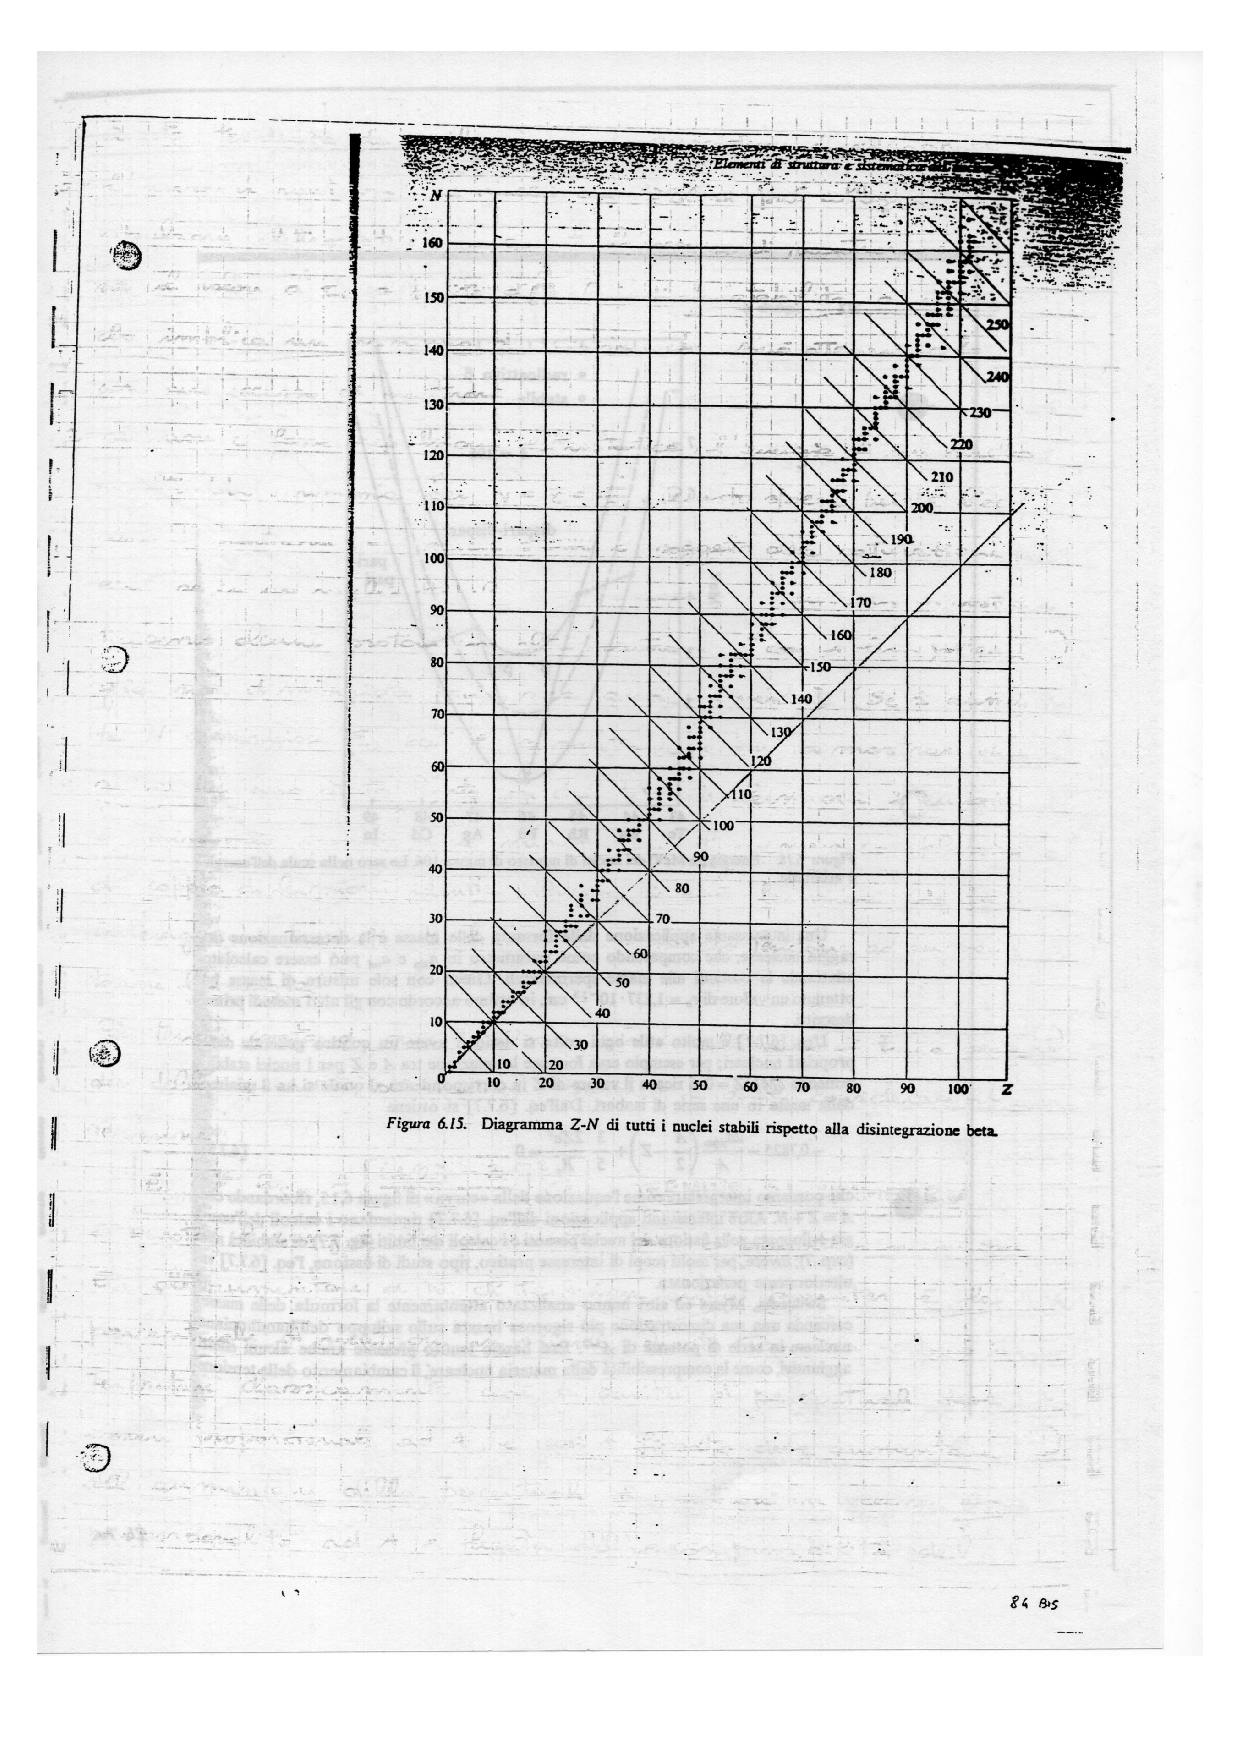
\includepdf[landscape,fitpaper=true,addtotoc={1,section,1,Allegato\
2,allegato_2}]{allegati/2.pdf}
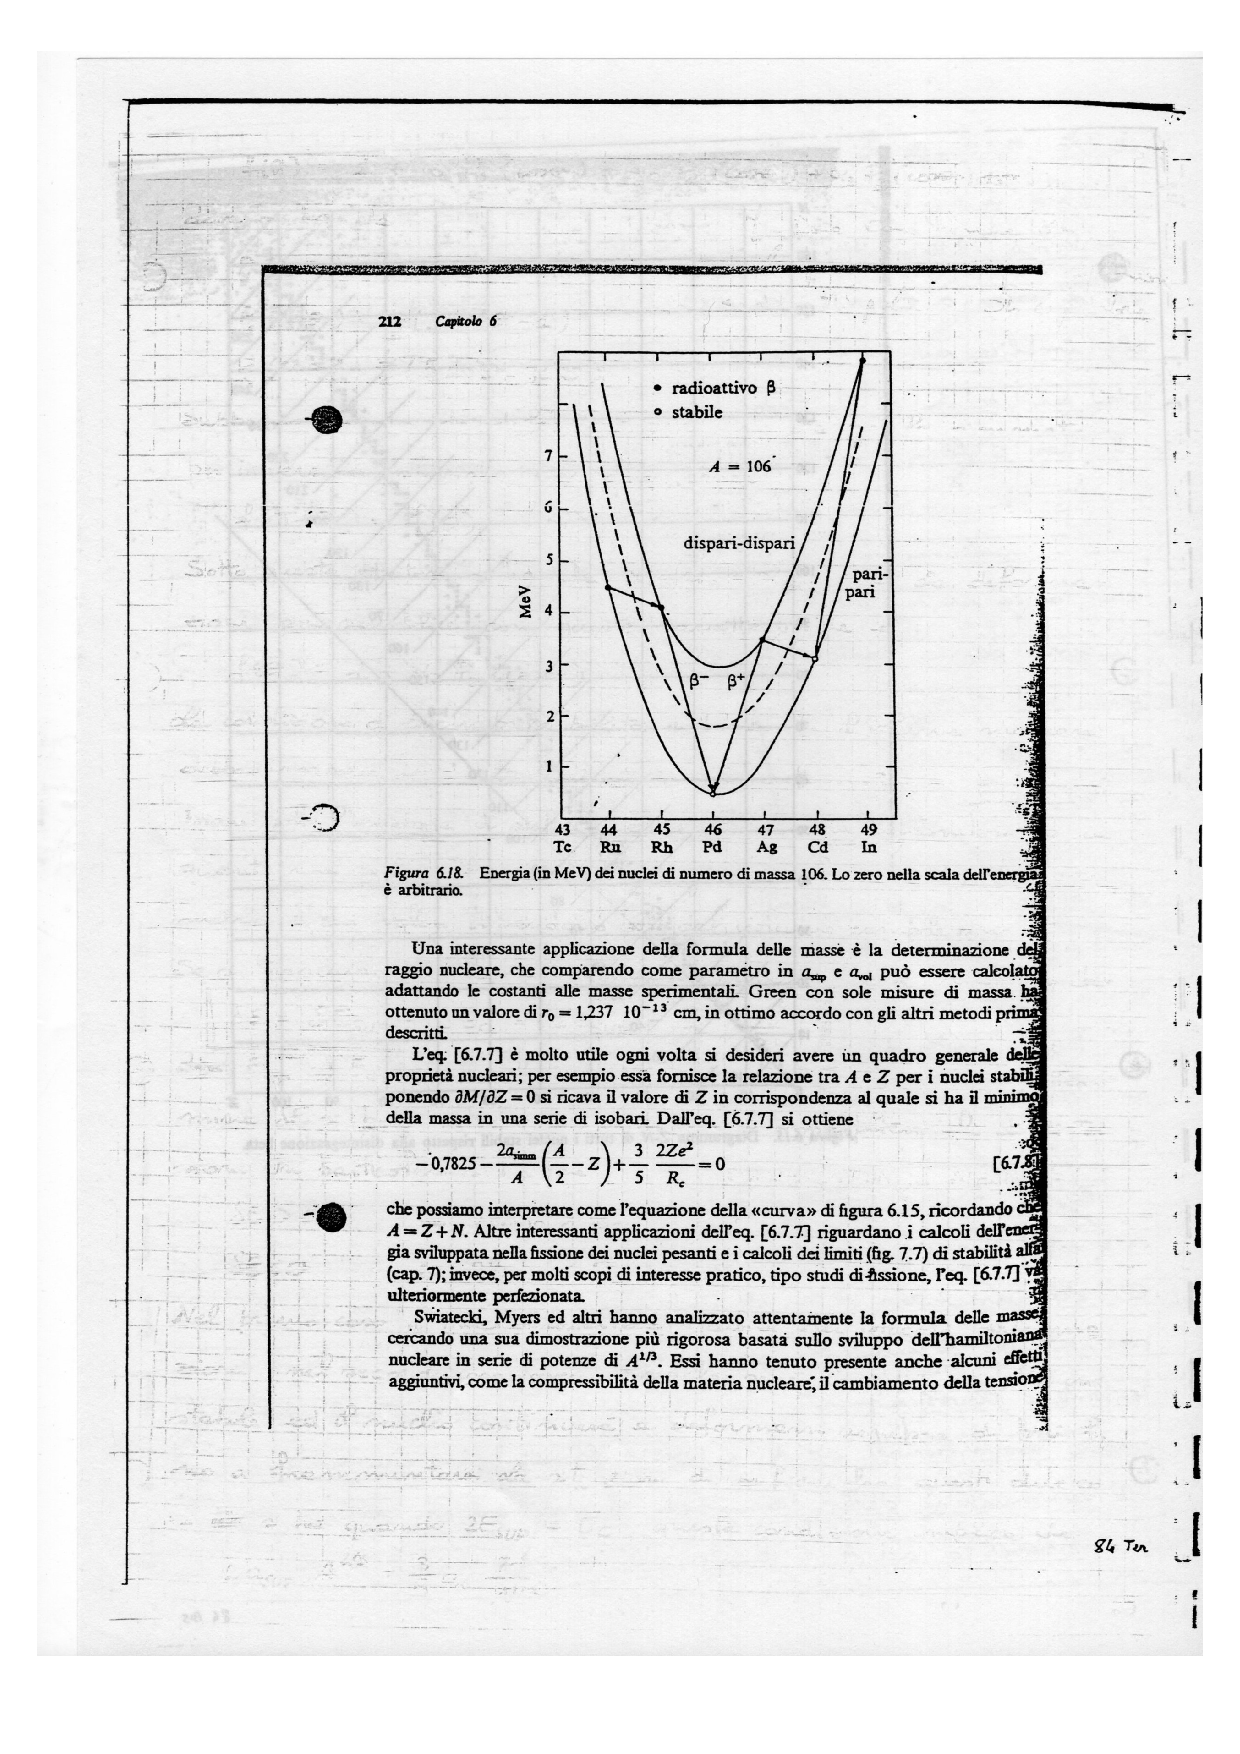
\includepdf[landscape,fitpaper=true,addtotoc={1,section,1,Allegato\
3,allegato_3}]{allegati/3.pdf}
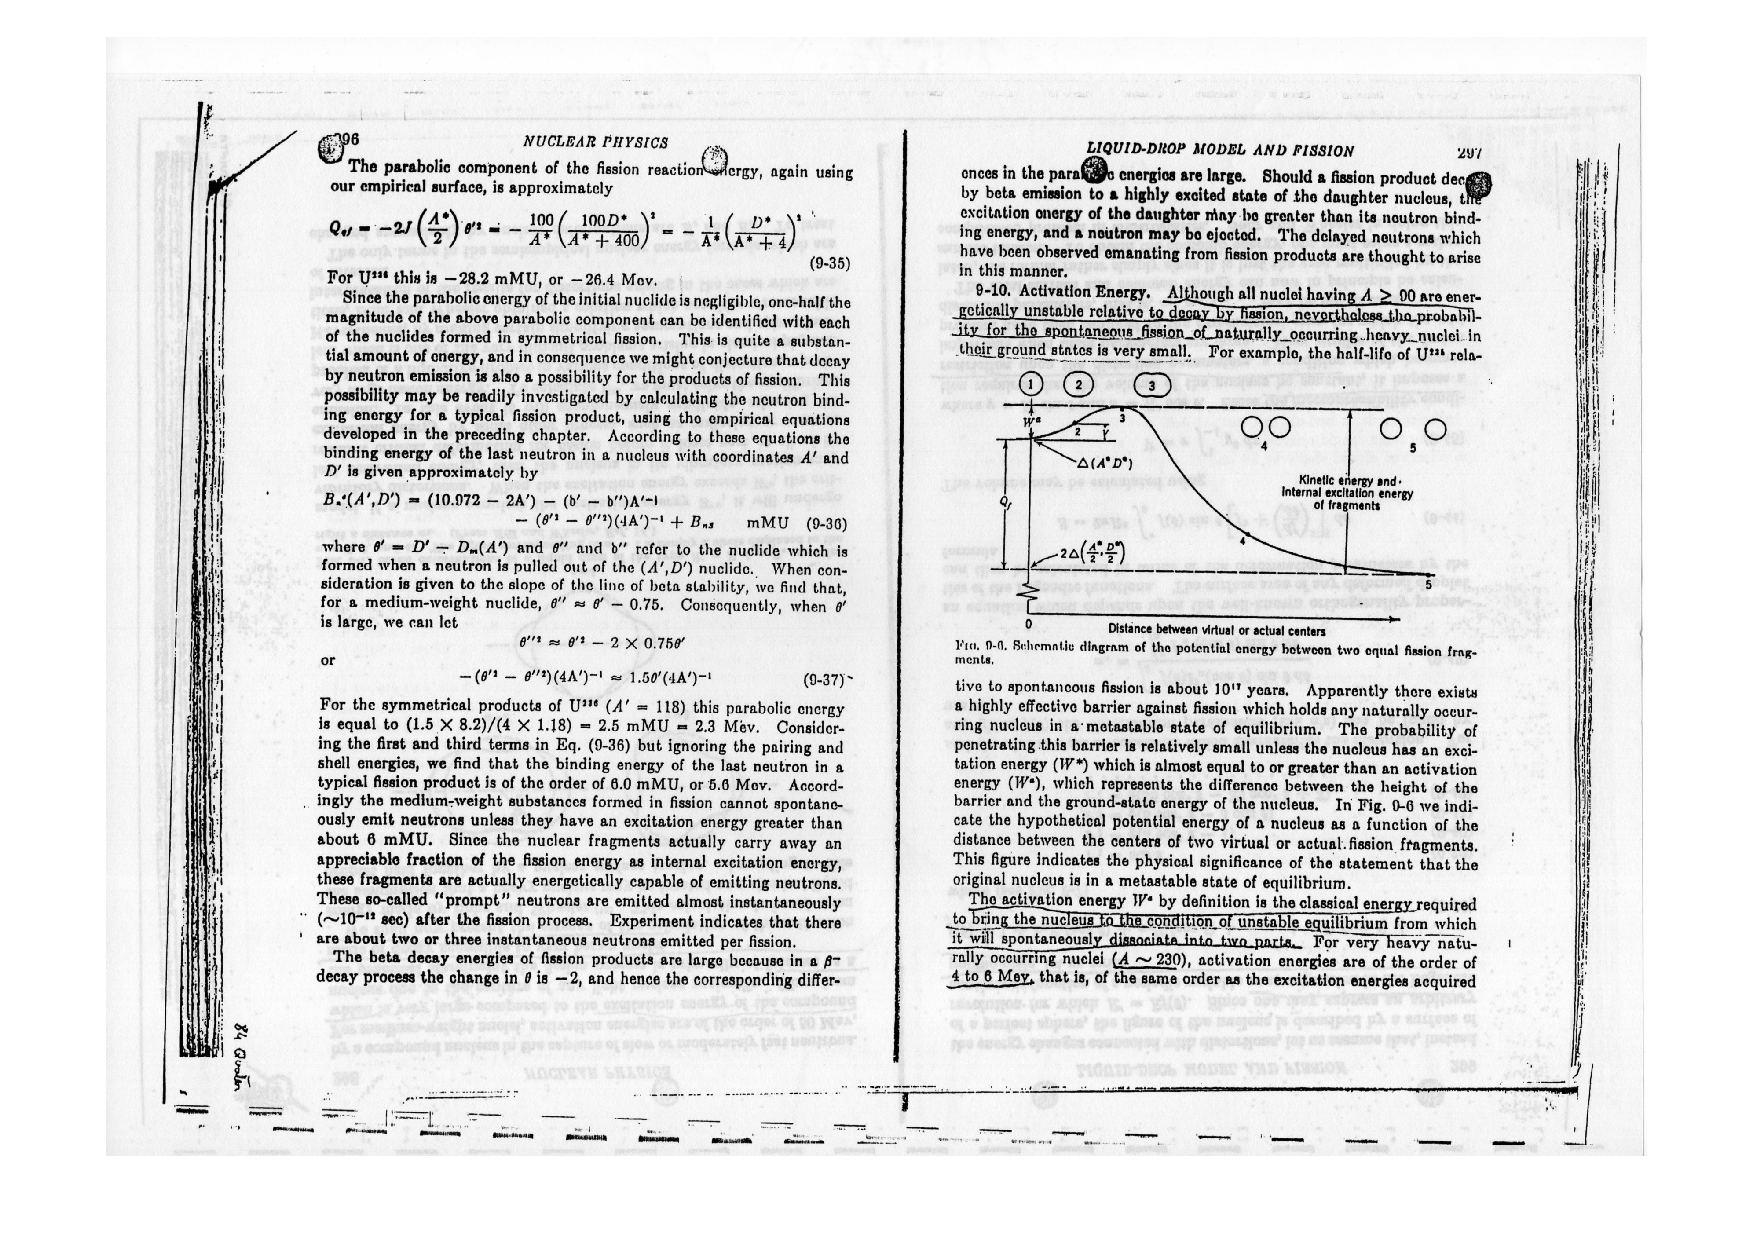
\includepdf[landscape,fitpaper=true,addtotoc={1,section,1,Allegato\
4(1),allegato_41}]{allegati/4_1.pdf}
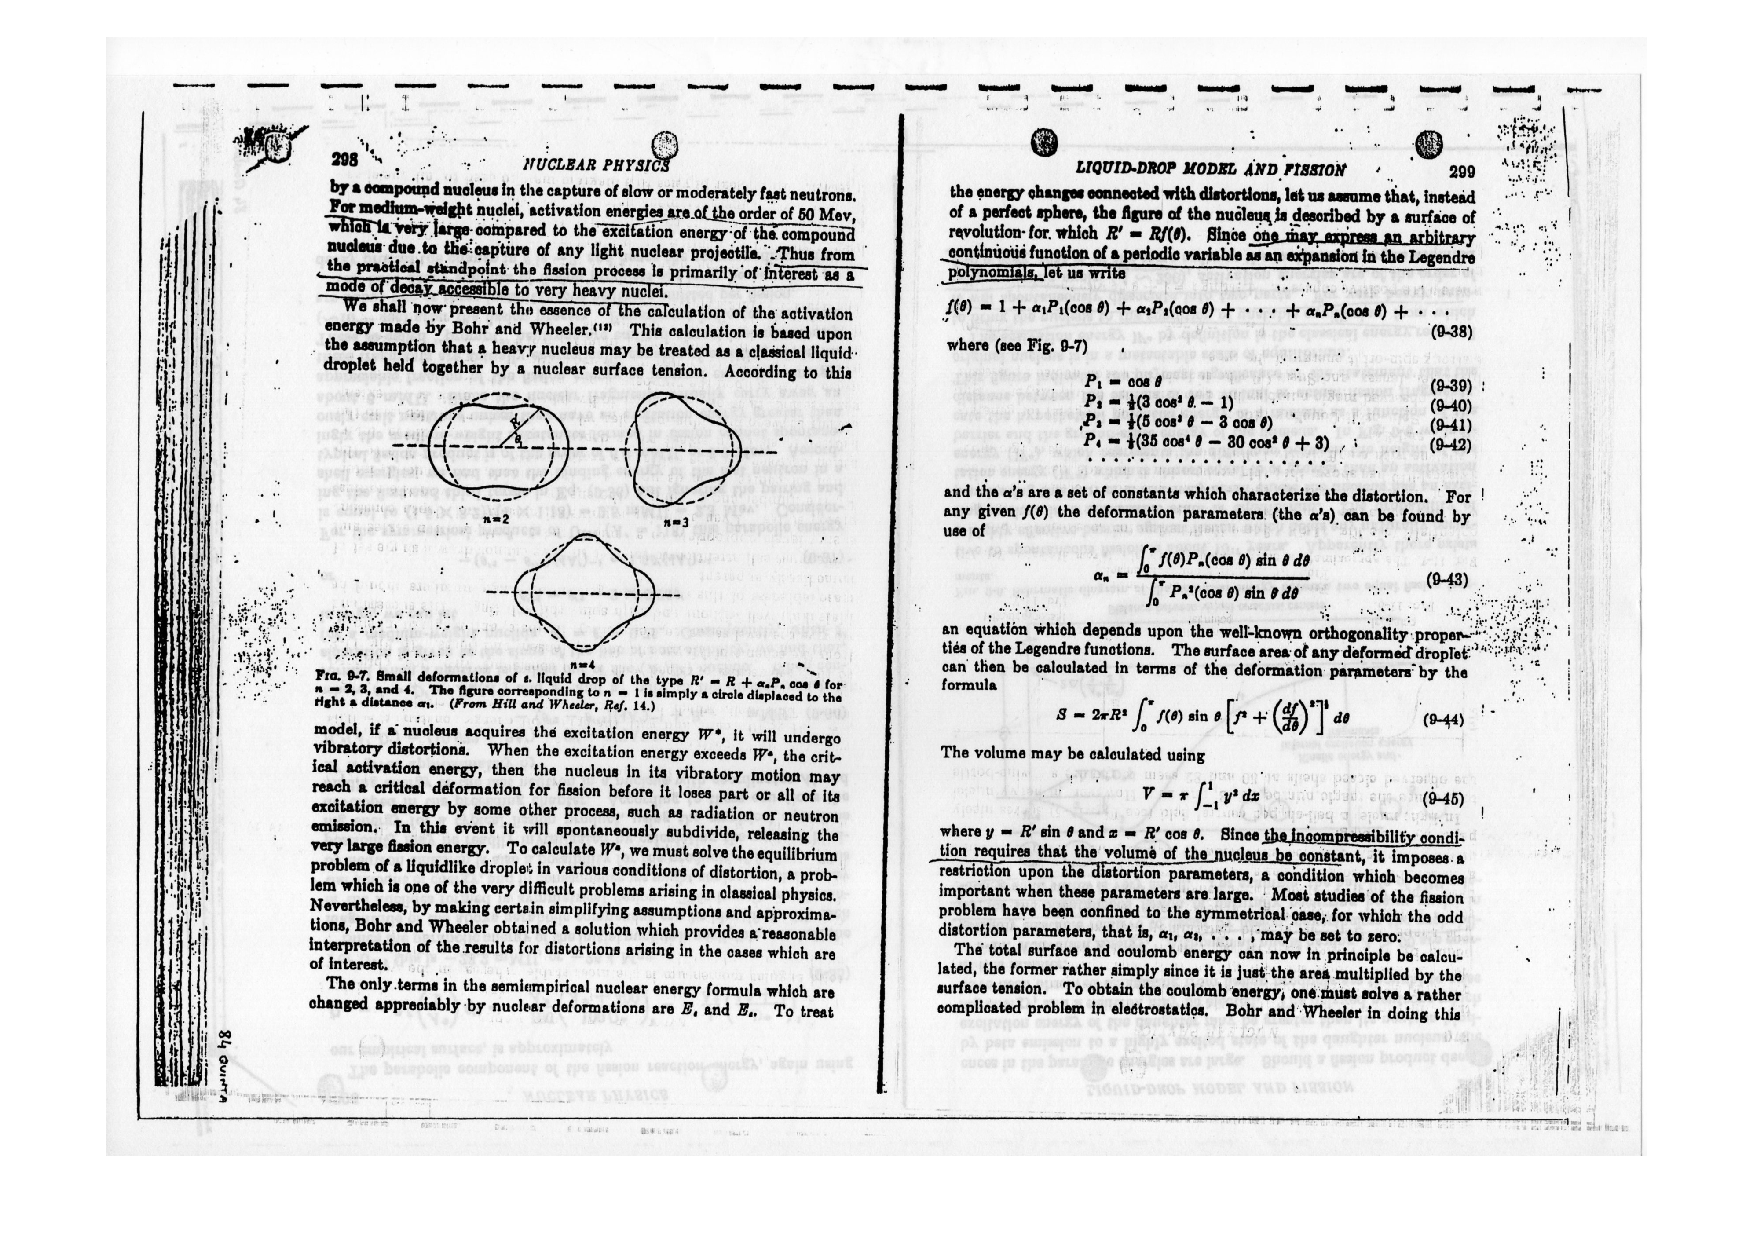
\includepdf[landscape,fitpaper=true,addtotoc={1,section,1,Allegato\
4(2),allegato_42}]{allegati/4_2.pdf}
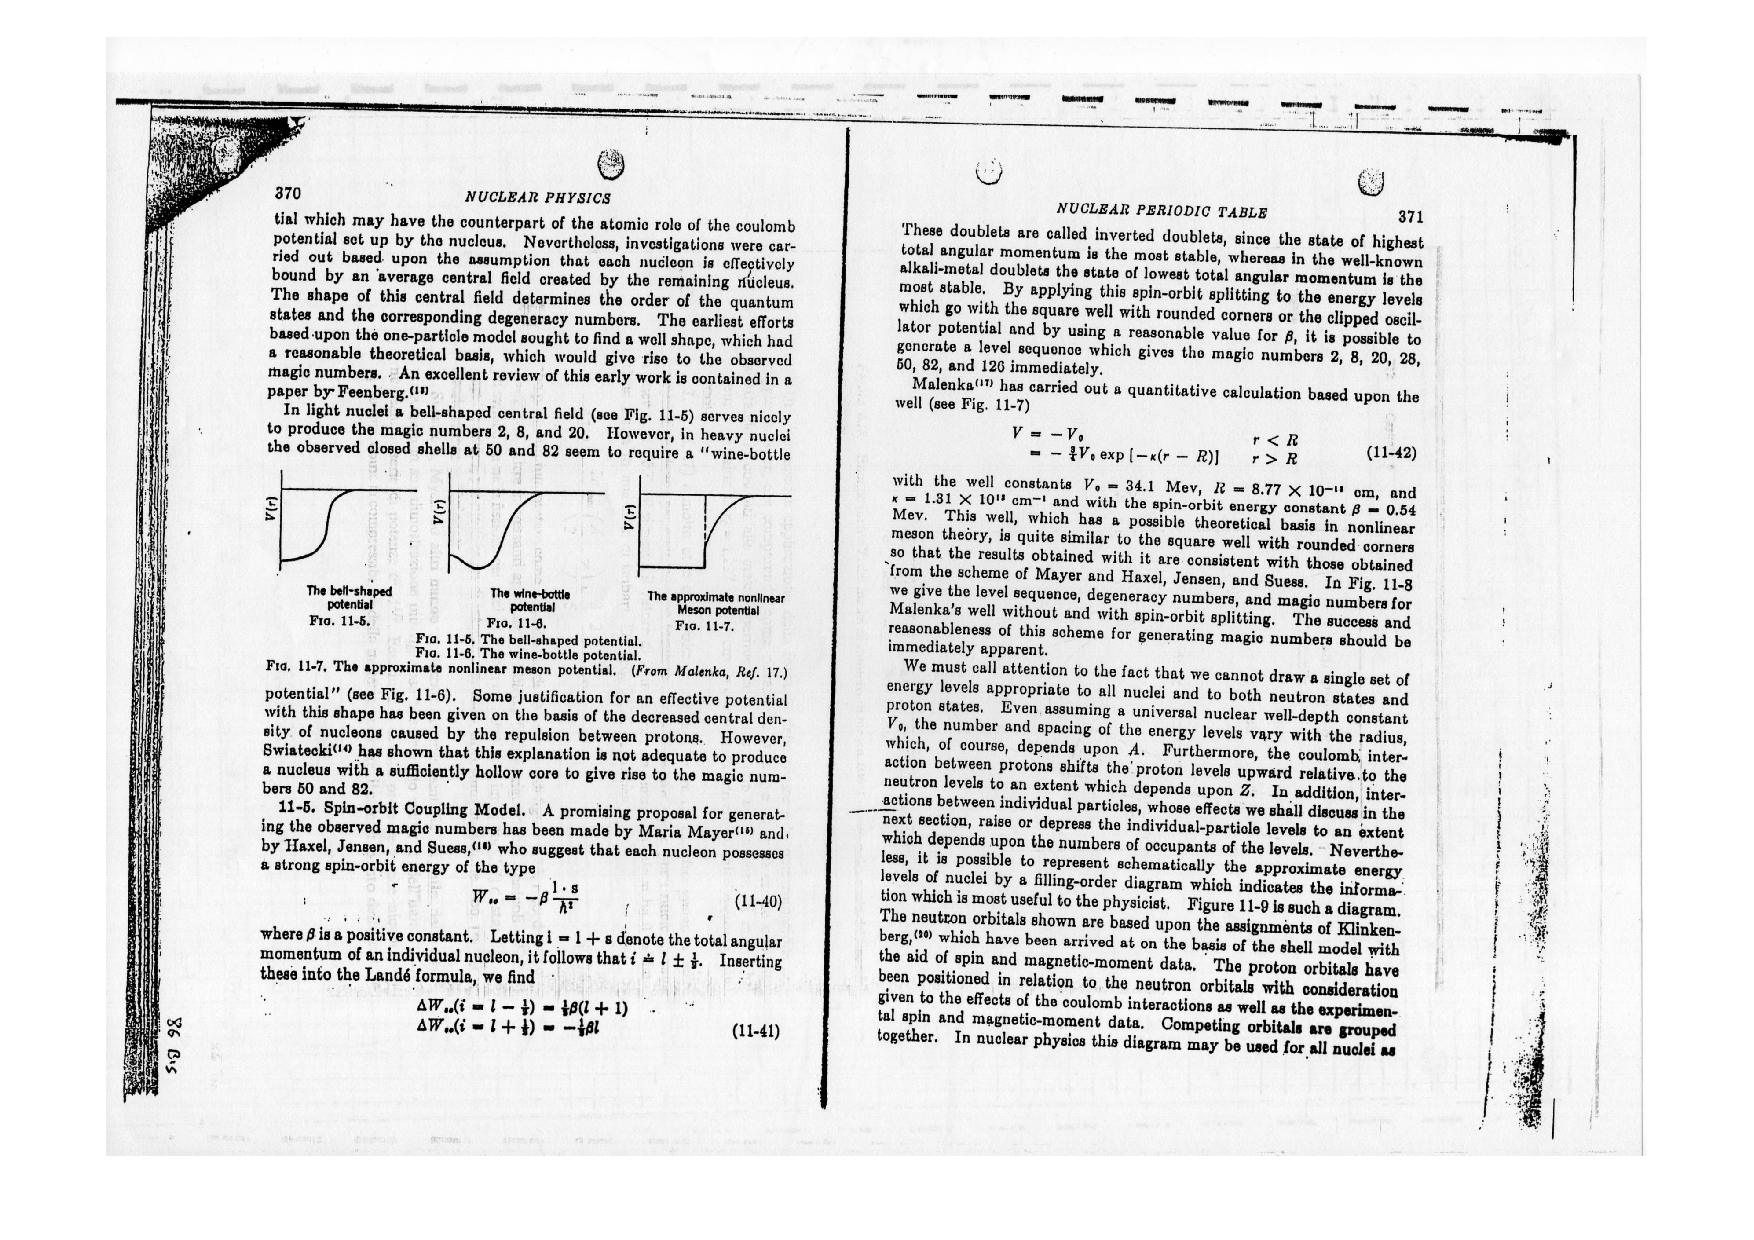
\includepdf[landscape,fitpaper=true,addtotoc={1,section,1,Allegato\
5,allegato_5}]{allegati/5.pdf}
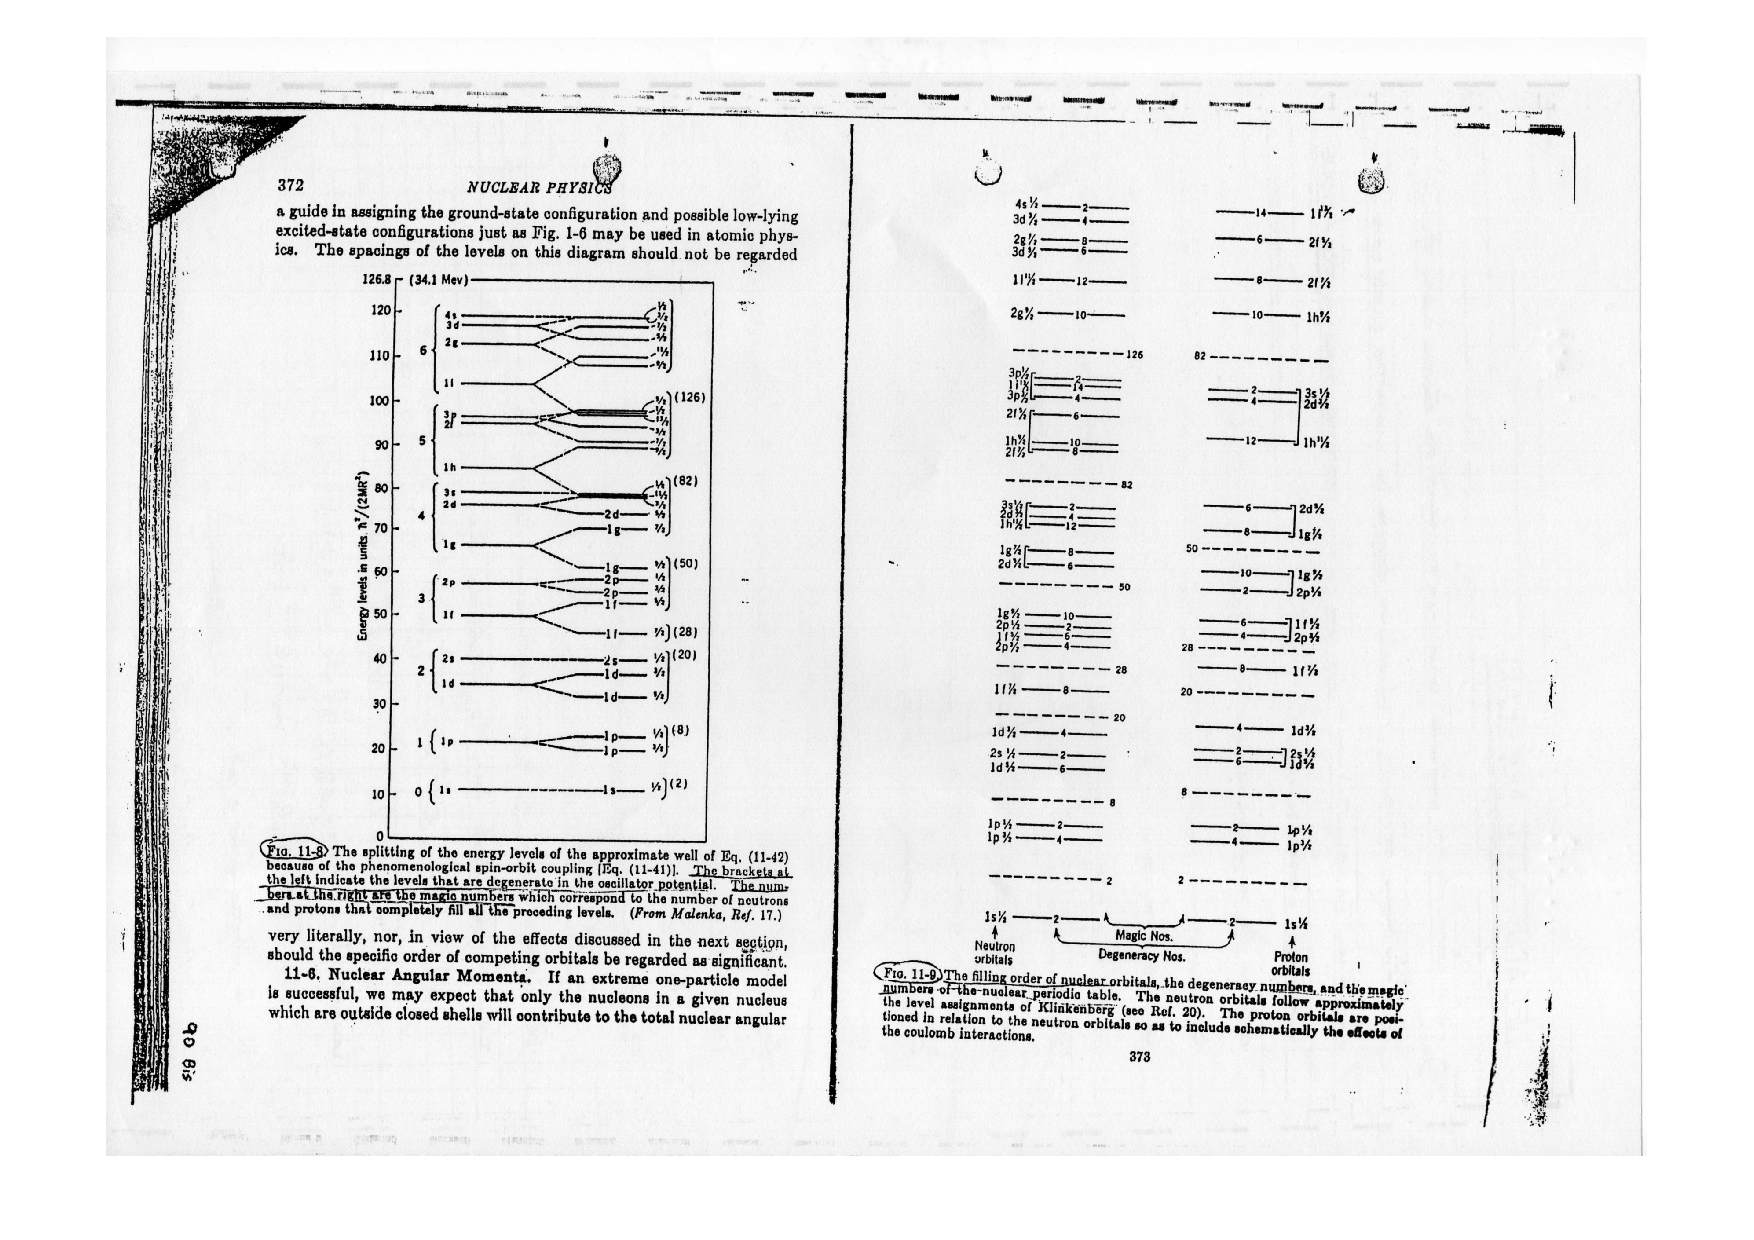
\includepdf[landscape,fitpaper=true,addtotoc={1,section,1,Allegato\
6,allegato_6}]{allegati/6.pdf}
